%!TEX root = ../main.tex

We show how to use \jilette for debugging JavaScript code annotated with 
separation logic (SL) specifications with the goal of finding bugs in both 
 specifications and code. In \S\ref{subsec:sep:assertions}, we describe the 
extension of the \jsil symbolic interpreter with a special construct for asserting
an SL-assertion. In \S\ref{specs:to:symbolic:tests}, we present an algorithm  
for generating symbolic tests from SL-specifications, so that if a 
symbolic test fails, the failure comes with a concrete counter-model that invalidates 
the specification. Finally, in \S\ref{specs:example}, we show how to use the 
proposed methodology for debugging JaVerT specifciations~\cite{javert} of JavaScript code. 

\subsection{\jsil Symbolic Execution with Separation Logic Assertions}
\label{subsec:sep:assertions}

We extend \jsil with a special construct, $\sepassert(P)$, for stating that 
the separation logic assertion $P$ must hold whenever $\sepassert(P)$ is evaluated. 
We make use of an adapted version of the assertion language from~\cite{javert}. 
In particular, instead of \emph{untyped logical variables}, we 
use \emph{typed logical variables}, $\svar \in \svars$, coinciding either with 
symbolic numbers, $\snumber \in \snumbers$, strings $\sstring \in \sstrings$, 
or locations, $\sloc \in \slocs$. 

\myparagraph{\jsil assertions: syntax and semantics}
\jsil assertions include: boolean operations; first-order connectives; the separating conjunction; 
existential quantification; and assertions for describing heaps. The $\lemp$ assertion describes 
an empty heap. The cell assertion, $(\lexpr_1,\lexpr_2) \pointsto \lexpr_3$,  describes an object 
at the location denoted by $\lexpr_1$ with a property denoted by $\lexpr_2$ that has the value 
denoted by $\lexpr_3$. The assertion $\emptyfields{\lexpr_1}{\lexpr_2}$ states that the object at 
the location denoted by $\lexpr_1$ has no properties other than possibly those included in the
set denoted by $\lexpr_2$. 
%
As in~\cite{gardner:popl:2012,javert}, in order to define the semantics of assertions, 
we resort to \emph{instrumented heaps} $\iheap \in \iheaps$, which differ from 
concrete heaps in that they may map object properties to the special value $\none$, 
explicitly indicating that the property does not exist (e.g. $\iheap(\loc, \jstring) = \none$
means that the object at location $\loc$ in the heap $\iheap$ does not have a property
named $\jstring$). 
%Analogously, we extend symbolic heaps with $\none$-cells, obtained \emph{instrumented symbolic heaps} $\isheap \in \isheaps$. 
Instrumented heaps are related to heaps by means of an \emph{erasure 
function}, $\deabstract{.}: \iheaps \rightarrow \heaps$, %($\deabstract{.}: \isheaps \rightarrow \sheaps$), 
which simply removes the none-cells from the instrumented heap given as input.  Below, we give the syntax and semantics of \jsil assertions. 

%  \deabstract{\jsilaheap}(\loc, x) = \jsilaheap(\loc, x) \iffdef (\loc, x) \in \domain(\jsilaheap) \ \wedge \ \jsilaheap(\loc, x) \neq \none

\begin{display}{\jsil Logic Assertions - syntax and semantics}
%
{\scriptsize \begin{tabular}{lll}
  %%%% 
  $\quad \lexpr \triangleq$ & $\lit \mid \jvar \mid \svar \mid \unoper\ \lexpr \mid \lexpr \binoper \lexpr$ &   \text{ Logical Expressions} \\[3pt]
  %%%%
  $\quad P\triangleq$ & $\jtrue \mid \jfalse \mid  \neg P \mid P \land P \mid P \lor P  \mid \lexpr = \lexpr \mid \lexpr \leq \lexpr$ & \text{ \polish{Pure Assertions}} \\
                                  & $\quad \mid \lemp \mid (\lexpr, \lexpr)\pointsto \lexpr \mid P \sep P  \mid \emptyfields{\lexpr}{\lexpr} $ &  \text{ Spatial Assertions} \\
\end{tabular}} \\ [7pt]
  %%%%%
  %%%%%
  
\quad 
{\scriptsize
\begin{tabular}{lll} 
     \begin{tabular}{ll}
    $\iheap, \store, \senv \satisfies \truep$                  &  $\Leftrightarrow \text{always}$   \\
    %
    $\iheap, \store, \senv \satisfies \falsep$                 &  $\Leftrightarrow \text{never}$   \\   
     %
    $\iheap, \store, \senv \satisfies \neg P$                 &  $\Leftrightarrow \iheap, \store, \env \not\satisfies P$ \\
     %  
     $\iheap, \store, \senv \satisfies P \land Q$           &  $ \Leftrightarrow \iheap, \store, \senv \satisfies P \land \iheap, \store, \senv \satisfies Q $   \\
     %   
     $\iheap, \store, \senv \satisfies  \exists \svar. P$  &  $\Leftrightarrow \exists \lit \in \lits. \, \iheap, \store, \senv[\svar \mapsto \lit] \satisfies P$  \\ 
     %  
      $\iheap, \store, \senv \satisfies \lexpr_1 = \lexpr_2$  &  $\Leftrightarrow \symbeval{\lexpr_1}{\store, \senv} = \symbeval{\lexpr_2}{\store, \senv}$   \\    
      %
      $\iheap, \store, \senv \satisfies \lexpr_1 \leq \lexpr_2$  &  $\Leftrightarrow \symbeval{\lexpr_1}{\store, \senv} \leq \symbeval{\lexpr_2}{\store, \senv}$   
      \end{tabular}
      &
      $\phantom{x}$
      &
       \begin{tabular}{l}
           $\iheap, \store, \senv  \satisfies  \lemp$ $\Leftrightarrow \iheap = \hemp$  \\[2pt]
           %
	   $\iheap, \store, \senv  \satisfies (\lexpr_1,\lexpr_2)\pointsto \lexpr_3$  \\
            $\ \Leftrightarrow \iheap =  \hcell{\symbeval{\lexpr_1}{\store, \senv}}{\symbeval{\lexpr_2}{\store, \senv}}{\symbeval{\lexpr_3}{\store, \senv}}$  \\[2pt]
           % 
           $\iheap, \store, \senv  \satisfies P \sep Q$ $\Leftrightarrow  \exists \iheap_1, \iheap_2.  \, \iheap = \iheap_1 \dunion \iheap_2$  \\
                $\qquad \wedge \ \iheap_1,  \store, \senv  \satisfies P \, \wedge \, \iheap_2,  \store, \senv \satisfies Q$ \\[2pt]
           %
           $\iheap, \store, \senv  \satisfies  \emptyfields{\lexpr_1}{\lexpr_2}$  \\
                $\ \Leftrightarrow \iheap = \biguplus_{s \not\in \{ \symbeval{\lexpr_2}{\store, \senv} \}} ((\symbeval{\lexpr_1}{\store, \senv}, s) \pointsto \none)$
           
       \end{tabular}
\end{tabular}}
\end{display}
%
For convenience, we define: 
{\small 
\begin{align}
\sepmodels{P} = \left\{ (\heap, \store) \mid \exists \iheap, \senv \, . \,  \heap = \deabstract{\iheap} \ \wedge \ \iheap, \store, \senv \satisfies P  \right\}
\end{align}}
\hspace{-2pt}Given a symbolic heap $\sheap$, a symbolic store $\sstore$, a path condition $\pc$, and 
an assertion $P$, we say that  $(\sheap, \sstore, \pc)$ \emph{satisfies} $P$, 
written $\sheap, \sstore, \pc \satisfies P$ \emph{if and only if}
$\smodels{\sheap, \sstore}{\pc} \subseteq \sepmodels{P}$. 
%
We can now give an \emph{ideal} symbolic semantics for the command $\sepassert(P)$ (which checks
if the current symbolic state satisfies $P$): 
{\small \begin{mathpar}
\inferrule[\textsc{Assert - True}]
  { 
     \sheap, \sstore, \pc \satisfies P
  }{\symbtrans{\sheap, \sstore, \sepassert(P), \pc}{\sheap, \sstore, \pc}} 
\and
\inferrule[\textsc{Assert - False}]
  { 
          \sheap, \sstore, \pc \not\satisfies P
  }{\symbtranserr{\sheap, \sstore, \sepassert(P), \pc}{}{\pc}} 
\end{mathpar}}
\hspace{-3pt}Determining whether or not a symbolic state satisfies an SL-assertion $P$ is, in general, 
undecidable. Importantly, since we do not want to produce \emph{false positives}, in order to trigger 
an assertion failure, we need to find a concrete witness for that failure. More precisely, when executing 
$\sepassert(P)$ in the symbolic state $(\sheap, \sstore, \pc)$, the symbolic analysis must  
report an assertion failure only if it can find a concrete state $(\heap, \store)$ such that: 
$(\heap, \store) \in \smodels{\sheap, \sstore}{\pc}$ and
$(\heap, \store) \not\in \sepmodels{P}$.

%\begin{figure}[t!]
%\centering
%{\scriptsize
%\begin{mathpar} 
%\inferrule[\textsc{New Existential}]
%     { 
%         \svar \in \existentials 
%         \quad
%         \svar \not\in \domain(\subst)
%     }
%     {\unification{\sexpr, \pc}{\svar}{\subst}{\existentials} = \uyes{\subst[\svar \mapsto \sexpr]}}
%\quad
%\inferrule[\textsc{Matched Existential}]
%     { 
%         \subst(\svar) = \sexpr' 
%         \quad 
%         \pc \vdash \sexpr = \sexpr' 
%     }
%     {\unification{\sexpr, \pc}{\svar}{\subst}{\existentials} = \uyes{\subst}}
%\quad
%\inferrule[\textsc{Existential - None}]
%     { 
%         \subst(\svar) = \sexpr' 
%         \quad 
%         \pc \not\vdash \sexpr = \sexpr' 
%     }
%     {\unification{\sexpr, \pc}{\svar}{\subst}{\existentials} = \uno{\sexpr \neq \sexpr'}}
%\\
%\inferrule[\textsc{Grounded Expression}]
%     { 
%         \fv(\subst(\sexpr')) \cap \existentials = \emptyset
%         \quad 
%          \pc \vdash  \sexpr = \subst(\sexpr') 
%     }
%     {\unification{\sexpr, \pc}{\sexpr'}{\subst}{\existentials} = \uyes{\subst}}
%\qquad
%\inferrule[\textsc{Grounded Expression - Fail}]
%     { 
%         \fv(\subst(\sexpr')) \cap \existentials = \emptyset
%         \quad 
%          \pc  \not\vdash  \sexpr = \subst(\sexpr') 
%     }
%     {\unification{\sexpr, \pc}{\sexpr'}{\subst}{\existentials} = \uno{\sexpr  \neq \subst(\sexpr')}}
%%
%\\
%%
%\\
%\inferrule[\textsc{None-Cell Assertion}]
%	{  
%	   \subst(\symbeval{\lexpr_l}{\sstore})  = \loc 
%	   \quad 
%	    \symbeval{\lexpr_p}{\sstore} = \sexprp' 
%	   \quad
%       \sheap = \sheap' \dunion  \big((l, \sexprp_i) \mapsto \sexprv_i\big)\mid_{i = 0}^n    
%	   \quad
%	   (l, -) \not\in \domain(\sheap')  
%	   \quad
%	    \pc \vdash \sexprp' \not\in \{ \sexprp_i \mid_{i = 0}^n \} 
%	}{ \unification{\sheap, \sstore, \pc}{(\lexpr_l,\lexpr_p)\pointsto \none}{\subst}{\existentials} = \uyes{\subst, \sheap}} 
%%
%\\
%\inferrule[\textsc{None-Cell Assertion - Fail}]
%	{  
%	   \subst(\symbeval{\lexpr_l}{\sstore})  = \loc 
%	   \quad 
%	    \symbeval{\lexpr_p}{\sstore} = \sexprp' 
%	   \quad
%       \sheap = \sheap' \dunion  \big((l, \sexprp_i) \mapsto \sexprv_i\big)\mid_{i = 0}^n    
%	   \quad
%	   (l, -) \not\in \domain(\sheap')  
%	   \quad
%	    \pc \not\vdash \sexprp' \not\in \{ \sexprp_i \mid_{i = 0}^n \} 
%	}{ \unification{\sheap, \sstore, \pc}{(\lexpr_l,\lexpr_p)\pointsto \none}{\subst}{\existentials} = \uno{\sexprp' \in \{ \sexprp_i \mid_{i = 0}^n \} }} 
%%
%\\
%\inferrule[\textsc{EmptyFields Assertion}]
%	{  
%	  \loc = \subst(\symbeval{\lexpr_l}{\sstore}) 
%	   \quad 
%	     \symbeval{\lexpr_d}{\sstore} = \sexprv' 
%	   \quad
%	     \sheap = \sheap' \, \uplus \, \big((l, \sexprp_i) \mapsto \sexprv_i\big)\mid_{i = 0}^n   
%              \quad
%             (l, -) \not\in \domain(\sheap')
%	    \quad 
%	    \pc \vdash \big( \{ \sexprp_i \mid_{i = 0}^n   \} \subseteq \sexprv' \big)
%	}{ \unification{\sheap, \sstore, \pc}{\emptyfields{\lexpr_l}{\lexpr_d}}{\subst}{\existentials} = \uyes{(\subst, \sheap)}} 
%\\
%\inferrule[\textsc{EmptyFields Assertion - Fail}]
%	{  
%	   \loc = \subst(\symbeval{\lexpr_l}{\sstore}) 
%	   \quad 
%	     \symbeval{\lexpr_d}{\sstore} = \sexprv' 
%	   \quad
%	     \sheap = \sheap' \, \uplus \, \big((l, \sexprp_i) \mapsto \sexprv_i\big)\mid_{i = 0}^n   
%              \quad
%             (l, -) \not\in \domain(\sheap')
%	    \quad 
%	    \pc \not\vdash \big( \{ \sexprp_i \mid_{i = 0}^n   \} \subseteq \sexprv' \big)
%	}{ \unification{\sheap, \sstore, \pc}{\emptyfields{\lexpr_l}{\lexpr_d}}{\subst}{\existentials} = \uno{\{ \sexprp_i \mid_{i = 0}^n   \} \not\subseteq \sexprv'}} 
%\end{mathpar}
%\hrule
%\caption{Unification of spatial assertions:
% {\scriptsize$\unification{\sheap, \sstore, \pc}{\cell}{\subst}{\existentials} = \uyes{\subst', \sheap_f} \texttt{ OR } \uno{\pc'}$}}\label{fig:unification}}
%\end{figure}

\myparagraph{Finding counter models for separation logic assertions}
We describe a partial decision procedure, which we  
implement as part of the \jsil symbolic interpreter, for proving entailments 
between symbolic states and SL-assertions \underline{and} finding counter 
models in case of failure.  
% I have to give more examples
As it is customary~\cite{javert}, the decision procedure works by first using \emph{pattern-matching} 
on the spatial part of the SL-assertion, and then discharging the pure part of the 
entailment to an external constraint solver (in our case, \rosette) . 

We target SL-assertions $P$ that can be represented as 4-tuples,
$(\existentials, \cells, \efs, \pfs)$, consisting of: 
\dtag{1} a set $\existentials$ of existentially quantified symbolic locations, 
\dtag{2} a list $\cells$ containing the non-none cell assertions (those whose value is different from $\none$), 
\dtag{3} a set $\efs$ containing the none-cell assertions and the empty-fields assertions, and
\dtag{4} a pure assertion $\pfs$. 
Hence, letting $\existentials = \{ \sloc_1, ..., \sloc_k \}$, $\cells = [ \cell_i \mid_{i = 0}^n ]$, and
$\efs = \{\efa_i \mid_{i = 0}^m \}$, we write $P \equiv (\existentials, \cells, \efs, \pfs)$ as shorthand for: 
{\small \begin{equation*}
P = \exists \sloc_1, ..., \sloc_k \, . \big( \bigoast_{0 \leq i \leq n} \cell_i \ \sep  \bigoast_{0 \leq i \leq m} \efa_i \big) \ \wedge \ \pfs
\end{equation*}}

\vspace{-10pt}
Given a symbolic state $(\sheap, \sstore, \pc)$ and an assertion $P \equiv (\existentials, \cells, \efs, \pfs)$, 
we represent each possible mapping from the existentially quantified symbolic locations in $P$ 
to the concrete locations in $\sheap$ as a \emph{substitution function} $\subst : \slocs \rightharpoonup \locs$.
Since both $\existentials$ and the set of concrete locations in $\sheap$ 
are finite, we conclude that there is a finite number of substitution functions to be considered 
when checking if $(\sheap, \sstore, \pc)$ satisfies $P$. 
%
Hence, in the following, we will assume a fixed substitution,~$\subst$. 

Below, we show the unification rules for non-none cell assertions. 
Unification of non-none cell assertions can either terminate
successfully with $\uyes{\sheap_f}$, in which case $\sheap_f$ denotes the
symbolic heap to be framed off, or unsuccessfully with $\uno{\pc'}$, 
in which case $\pc'$ captures the constraints that need to hold for 
the entailment no to hold.
Given a cell assertion $\cell$, a symbolic state $(\sheap, \pc)$, 
and a substitution $\subst$: 
\begin{itemize}
    \item if $\unification{\sheap, \pc}{\cell}{} = \uyes{\sheap_f}$, then there are 
            two heaps $\sheap'$ and $\sheap_f$, such that $\sheap = \sheap' \dunion \sheap_f$
            and $\smodels{\sheap', -}{\pc} \subseteq \sepmodels{\cell}$; 
   
   \item if $\unification{\sheap, \pc}{\cell}{} = \uno{\pc'}$, then there are 
            no two heaps $\sheap'$ and $\sheap_f$, such that $\sheap = \sheap' \dunion \sheap_f$ 
            and $\smodels{\sheap', -}{\pc \, \wedge \, \pc'} \subseteq \sepmodels{\cell}$.
\end{itemize}



\vspace{-3pt}
\begin{display}{Unification of non-none cell assertions: $\unification{\sheap, \pc}{\cell}{} = \uyes{\sheap_f} \texttt{ or } \uno{\pc'}$}
{\scriptsize
\begin{mathpar} 
\inferrule[\textsc{Cell Assertion}]
	{  
	   \cell = (\loc,\sexprp)\pointsto \sexprv 
	   \\\\
	    \sheap = \sheap_f \dunion ((l, \sexprp') \mapsto \sexprv') 
	   \\\\
	    \pc \vdash  \sexprp = \sexprp' \wedge \sexprv = \sexprv'
	}{ \unification{\sheap, \pc}{\cell}{} = \uyes{\sheap_f}} 
\quad
\inferrule[\textsc{Cell Assertion - Fail}]
	{  
	   \cell = (\loc,\sexprp)\pointsto \sexprv \quad
	   \sheap = \sheap' \dunion  \big((l, \sexprp_i) \mapsto \sexprv_i\big)\mid_{i = 0}^n  
	    \\\\ 
	     l \notin \hlocs{\sheap'}
	     \quad
	    \pc_i = (\sexprp_i = \sexprp' \wedge \sexprv_i = \sexprv')\!\mid_{i = 0}^n
	    \quad
	    \pc \not\vdash \pc_i \mid_{i = 0}^n
	}{ \unification{\sheap, \pc}{\cell}{} = 
		\uno{\wedge_{0 \leq i \leq n} \neg\pc_i}} 
\quad
\inferrule[\textsc{Iterated-CU}]
	{  
	   \unification{\sheap, \pc}{\cell}{} = \uyes{\sheap_f}
	}{\cellunification{\sheap, \cell \lstcons \cells}{\sheap_f, \cells}\pc}
\end{mathpar}}
\end{display}


%\vspace{-3pt}
%\begin{display}{Unification of negative-resource assertions: $\unificationef{\sheap}{\efs} = \pc$ and $\sanity{\efs} = \pc$}
\begin{figure}
{\scriptsize
\begin{mathpar} 
\inferrule[\textsc{None Cell Assertion}]
	{  
	   \sheap = \sheap' \, \uplus \, \big((l, \sexprp_i) \mapsto -\big)\mid_{i = 0}^n   
	   \ 
	    l \notin \hlocs{\sheap'}
	 }{ \unificationefl{\sheap}{(\loc,\sexprp)\pointsto \none} = \sexprp \not\in \{  \sexprp_i \mid_{i = 0}^n \} }
\qquad
\inferrule[\textsc{Empty Fields Assertion}]
	{  
	    \sheap = \sheap' \dunion  \big((l, \sexprp_i) \mapsto -\big)\mid_{i = 0}^n   
	    \ 
	     l \notin \hlocs{\sheap'}
	}{ \unificationefl{\sheap}{\emptyfields{\loc}{\sexpr_d}}{} =  \{ \sexprp_i \mid_{i = 0}^n \} \subseteq \sexpr_d   } 
\\
%
\inferrule[\textsc{Sanity Constraints - Fixed Location}]
	{
		 \efproj{\efs}{\loc} = \emptyfields{\loc}{\sexpr_d} \sep  \oast_{i = 0}^{n} \, \big((l, \sexprp_i) \mapsto \none \big)
	}{ \sanityl{\efs}{\loc} = 
		 (\wedge_{0 \leq i, j \leq n, i \neq j} \sexprp_i \neq \sexprp_j)
		       \, \wedge \,  ( \wedge_{0 \leq i \leq n} \sexprp_i \notin \sexpr_d )
	} 
%
\\
\inferrule[\textsc{Negative Resource Unification}]
	{}{ \unificationef{\sheap}{\efs} =  \bigwedge_{\efa \in \efs}  \unificationefl{\sheap}{\efa}} 
\and
\inferrule[\textsc{Sanity Constraints}]
	{}{ \sanity{\efs} = \bigwedge_{\loc \in \eflocs(\efs)}\sanityl{\efs}{\loc}} 
\end{mathpar}}
\caption{Unification of negative-resource assertions: $\unificationef{\sheap}{\efs} = \pc$ and $\sanity{\efs} = \pc$}
\end{figure}


\begin{figure}[t!]
{\scriptsize
\centering
\begin{mathpar} 
\inferrule[\textsc{Success}]
	{     
	   \cellunificationiter{\sheap, \cells}{\hemp, []}{\pc}
	   \quad 
	   \pc'' = \unificationef{\sheap}{\efs} 
	   \\\\
	   \pc''' = \sanity{\efs} 
	   \quad
	   \pc \vdash \pfs' \, \wedge \, \pc''  \, \wedge \, \pc'''
	}{\unificationfull{\sheap, \pc}{\cells, \efs, \pfs'}{}} 
\and
\inferrule[\textsc{Fail - Pure Entailment}]
	{  
	   \cellunificationiter{\sheap, \cells}{\hemp, []}{\pc}
	   \quad 
	   \pc'' = \unificationef{\sheap}{\efs} 
	   \\\\
	    \pc''' = \sanity{\efs} 
	    \quad
             \pc \not\vdash \pfs' \, \wedge \, \pc'' \wedge \, \pc'''
	}{\unificationfullfail{\sheap, \pc}{\cells, \efs, \pfs'}{}{\neg(\pc'  \, \wedge \, \pc'' \wedge \, \pc''')}} 
\\
%
\inferrule[\textsc{Fail - Extra Resource}]
	{  
	     \cellunificationiter{\sheap, \cells}{\sheap_f, []}{\pc}
	     \qquad
	     \sheap_f \neq \hemp
	}{\unificationfullfail{\sheap, \pc}{\emptyset, \efs, \pfs'}{}{\jtrue}} 
%
\and
%
\inferrule[\textsc{Fail - Cell Unification}]
	{  
	   \cellunificationiter{\sheap, \cells}{\sheap', \cell \lstcons -}{\pc}
            \qquad
          \unification{\sheap', \pc}{\cell}{} = \uno{\pc''}
	}{\unificationfullfail{\sheap, \pc}{\cells, \efs, \pfs'}{}{\pc''}} 
\end{mathpar}}
\hrule
\caption{Unification algorithm: {\small $\unificationfull{\sheap, \pc}{\cells, \pfs'}{}$}
and {\small $\unificationfullfail{\sheap, \pc}{\cells, \pfs'}{}{\pc'}$}.\label{unification:algorithm}}
\end{figure}

Figure~\ref{unification:algorithm} presents the rules for the \emph{unification algorithm}. 
\polish{Notation not given?}
The algorithm works by trying to unify the non-none cell assertions first. If they are all 
successfully unified and the resulting symbolic heap is empty, then the final pure entailment 
is discharged to the constraint solver. If the resulting symbolic heap is non-empty, then there 
is additional resource and the unification also fails. Note that in case of failure, the algorithm 
returns the constraints that need to be satisfied for a witness of that failure to be produced. 

The soundness of unification theorem states that: given an SL-assertion $P$ and a 
symbolic state $(\sheap, \sstore, \pc)$, if we find a substitution $\subst$ 
for which the unification algorithm terminates successfully; then the symbolic state
$(\sheap, \sstore, \pc)$ satisfies $P$. 
The bug-finding theorem is more subtle. It states that: if for all possible substitutions 
$\subst$, the unification algorithm terminates with failure; then, in order to find a counter-model 
for $P$, we just have to pick a concretisation of the symbolic state that is consistent with all 
the failing constraints. Below, we use $\substs(\existentials, \sheap)$ to denote 
the set of all mappings from $\existentials$ to the locations in~$\sheap$. 

\begin{theorem}[Soundness of Unification]\label{teo:unification:soundness}
$\forall P, \cells, \efs, \pfs',  \sheap, \sstore, \pc, \subst \, .$
$$
\begin{array}{l}
\symbeval{\subst(P)}{\sstore} \equiv (\emptyset, \cells, \efs, \pfs') \ \wedge \ \unificationfull{\sheap, \pc}{\cells, \efs, \pfs'}{} \
    \implies \smodels{\sheap, \sstore}{\pc} \subseteq \sepmodels{P}   
\end{array}
$$ 
\end{theorem}


\begin{theorem}[Bug-finding for SL]
$\forall P, \existentials, \cells, \efs, \pfs', \subst_k\!\mid_{k=0}^n,\sheap, \sstore, \pc \, .$
$$
\begin{array}{l}
   P \equiv (\existentials, -, -, -) \implies \substs(\existentials, \sheap) = \{ \subst_k \mid_{k=0}^n \} \implies  \\
   \qquad \forall_{0 \leq k \leq n} \, . \, \big(
   \symbeval{\subst_k(P)}{\sstore} \equiv (\emptyset, \cells, \efs, \pfs') 
       \implies \\
  \qquad \qquad \unificationfullfail{\sheap, \sstore, \pc}{\cells, \efs, \pfs'}{}{\pc_k} \implies \smodels{\sheap, \sstore}{\pc''} \cap \sepmodels{P} = \emptyset   \big)
\end{array}
$$ 
for $\pc'' = \pc \, \wedge \, \bigwedge_{k=0}^{n} \pc_k$.
\end{theorem}


\newpage
\subsection{Compiling \jsil Specifications to Symbolic Tests}
\label{specs:to:symbolic:tests}
\polish{Explain \jsil specs} 

\begin{definition}[Validity of \jsil Logic Specifications]
A \jsil logic specification $\lconf{P} \, \fid(\jvec{x}) \,  \lconf{Q}$ for return mode $\flag$ is valid with respect to a program 
$\prog$, written $\prog, \flag \vDash \lconf{P} \, \fid(\jvec{x}) \,  \lconf{Q}$,  if and only if, for all logical 
contexts $(\iheap, \store, \senv)$, heaps $\heap_f$, stores $\store_f$, and flags $\flag'$, it holds that: 
$$
\begin{array}{l}
    \iheap, \store, \senv \satisfies P \ \wedge \ \tuple{\deabstract{\iheap}, \store, \ctx[0]} \rightarrow^* \tuple{\heap_f, \store_f, \ctx[i_{\flag'}]} \\
       \quad \implies
            \flag' = \flag \ \wedge \ \exists \iheap_f \, . \, \iheap_f, \store_f, \senv \satisfies Q \ \wedge \ \deabstract{\iheap_f} = \heap_f
\end{array}
$$
\end{definition}

\noindent Given a \jsil program $\prog$ containing a procedure $\fid$ with spec {\small $\lconf{P} \, \fid(\jvec{x}) \,  \lconf{Q}$}, 
our goal is to construct a symbolic test for checking whether or not $\fid$ behaves as its specification mandates.
A symbolic test is a pair $(\prog', \sheap)$ consisting of a \jsil program and a symbolic heap. The new program $\prog'$ 
differs from $\prog$ in that it has a new \jsilmain procedure with the code of the test, and $\sheap$ is the initial 
symbolic heap on which to execute $\prog'$. 

\begin{display}{Concretisation of \jsil assertions: $\concretise{\cell}{\subst} = \sheap, \subst'$ and $\concretise{(\existentials, \sfs, \pfs)}{\subst} = \sheap, \pfs', \subst'$}
{\scriptsize
\begin{mathpar} 
\inferrule[\textsc{Spatial Assertion - Lit Loc}]
	{
	  \concretise{\lexpr_p}{\subst} = \sexpr_p, \subst' 
	  \quad 
	  \concretise{\lexpr_v}{\subst'} = \sexpr_v, \subst''
	}{\concretise{(\loc,\lexpr_p)\pointsto \lexpr_v}{\subst} = (\loc,\sexpr_p)\pointsto \sexpr_v, \subst''}  
\and 
\inferrule[\textsc{Spatial Assertion - Var Loc}]
	{
	  \concretise{\lexpr_p}{\subst[\sloc \mapsto \loc]} = \sexpr_p, \subst' 
	  \quad 
	  \concretise{\lexpr_v}{\subst'} = \sexpr_v, \subst''
	  	  \quad 
	  \loc \ \cfresh
	}{\concretise{(\sloc,\lexpr_p)\pointsto \lexpr_v}{\subst} = (\loc,\sexpr_p)\pointsto \sexpr_v, \subst''}  
\and 
\inferrule[\textsc{EmptyFileds}]
	{}{\concretise{\emptyfields{-}{-}}{\subst} = \hemp, \subst}  
\and 
\inferrule[\textsc{Spatial Assertion}]
	{
	    \sfs = \{ \cell \} \dunion \sfs'
	    \quad 
	    \concretise{\cell}{\subst} = \sheap, \subst' 
	    \\\\
	    \concretise{(-, \sfs', \pfs)}{\subst'} = \sheap', \pfs', \subst''
	}{\concretise{(-, \sfs, \pfs)}{\subst} = \sheap \dunion \sheap', \pfs', \subst''}  
\and 
\inferrule[\textsc{Spatial Assertion}]
	{
	}{\concretise{(-, \emptyset, \pfs)}{\subst} = \hemp, \subst(\pfs), \subst}  
\end{mathpar}}
\end{display}

\begin{figure}[t!]
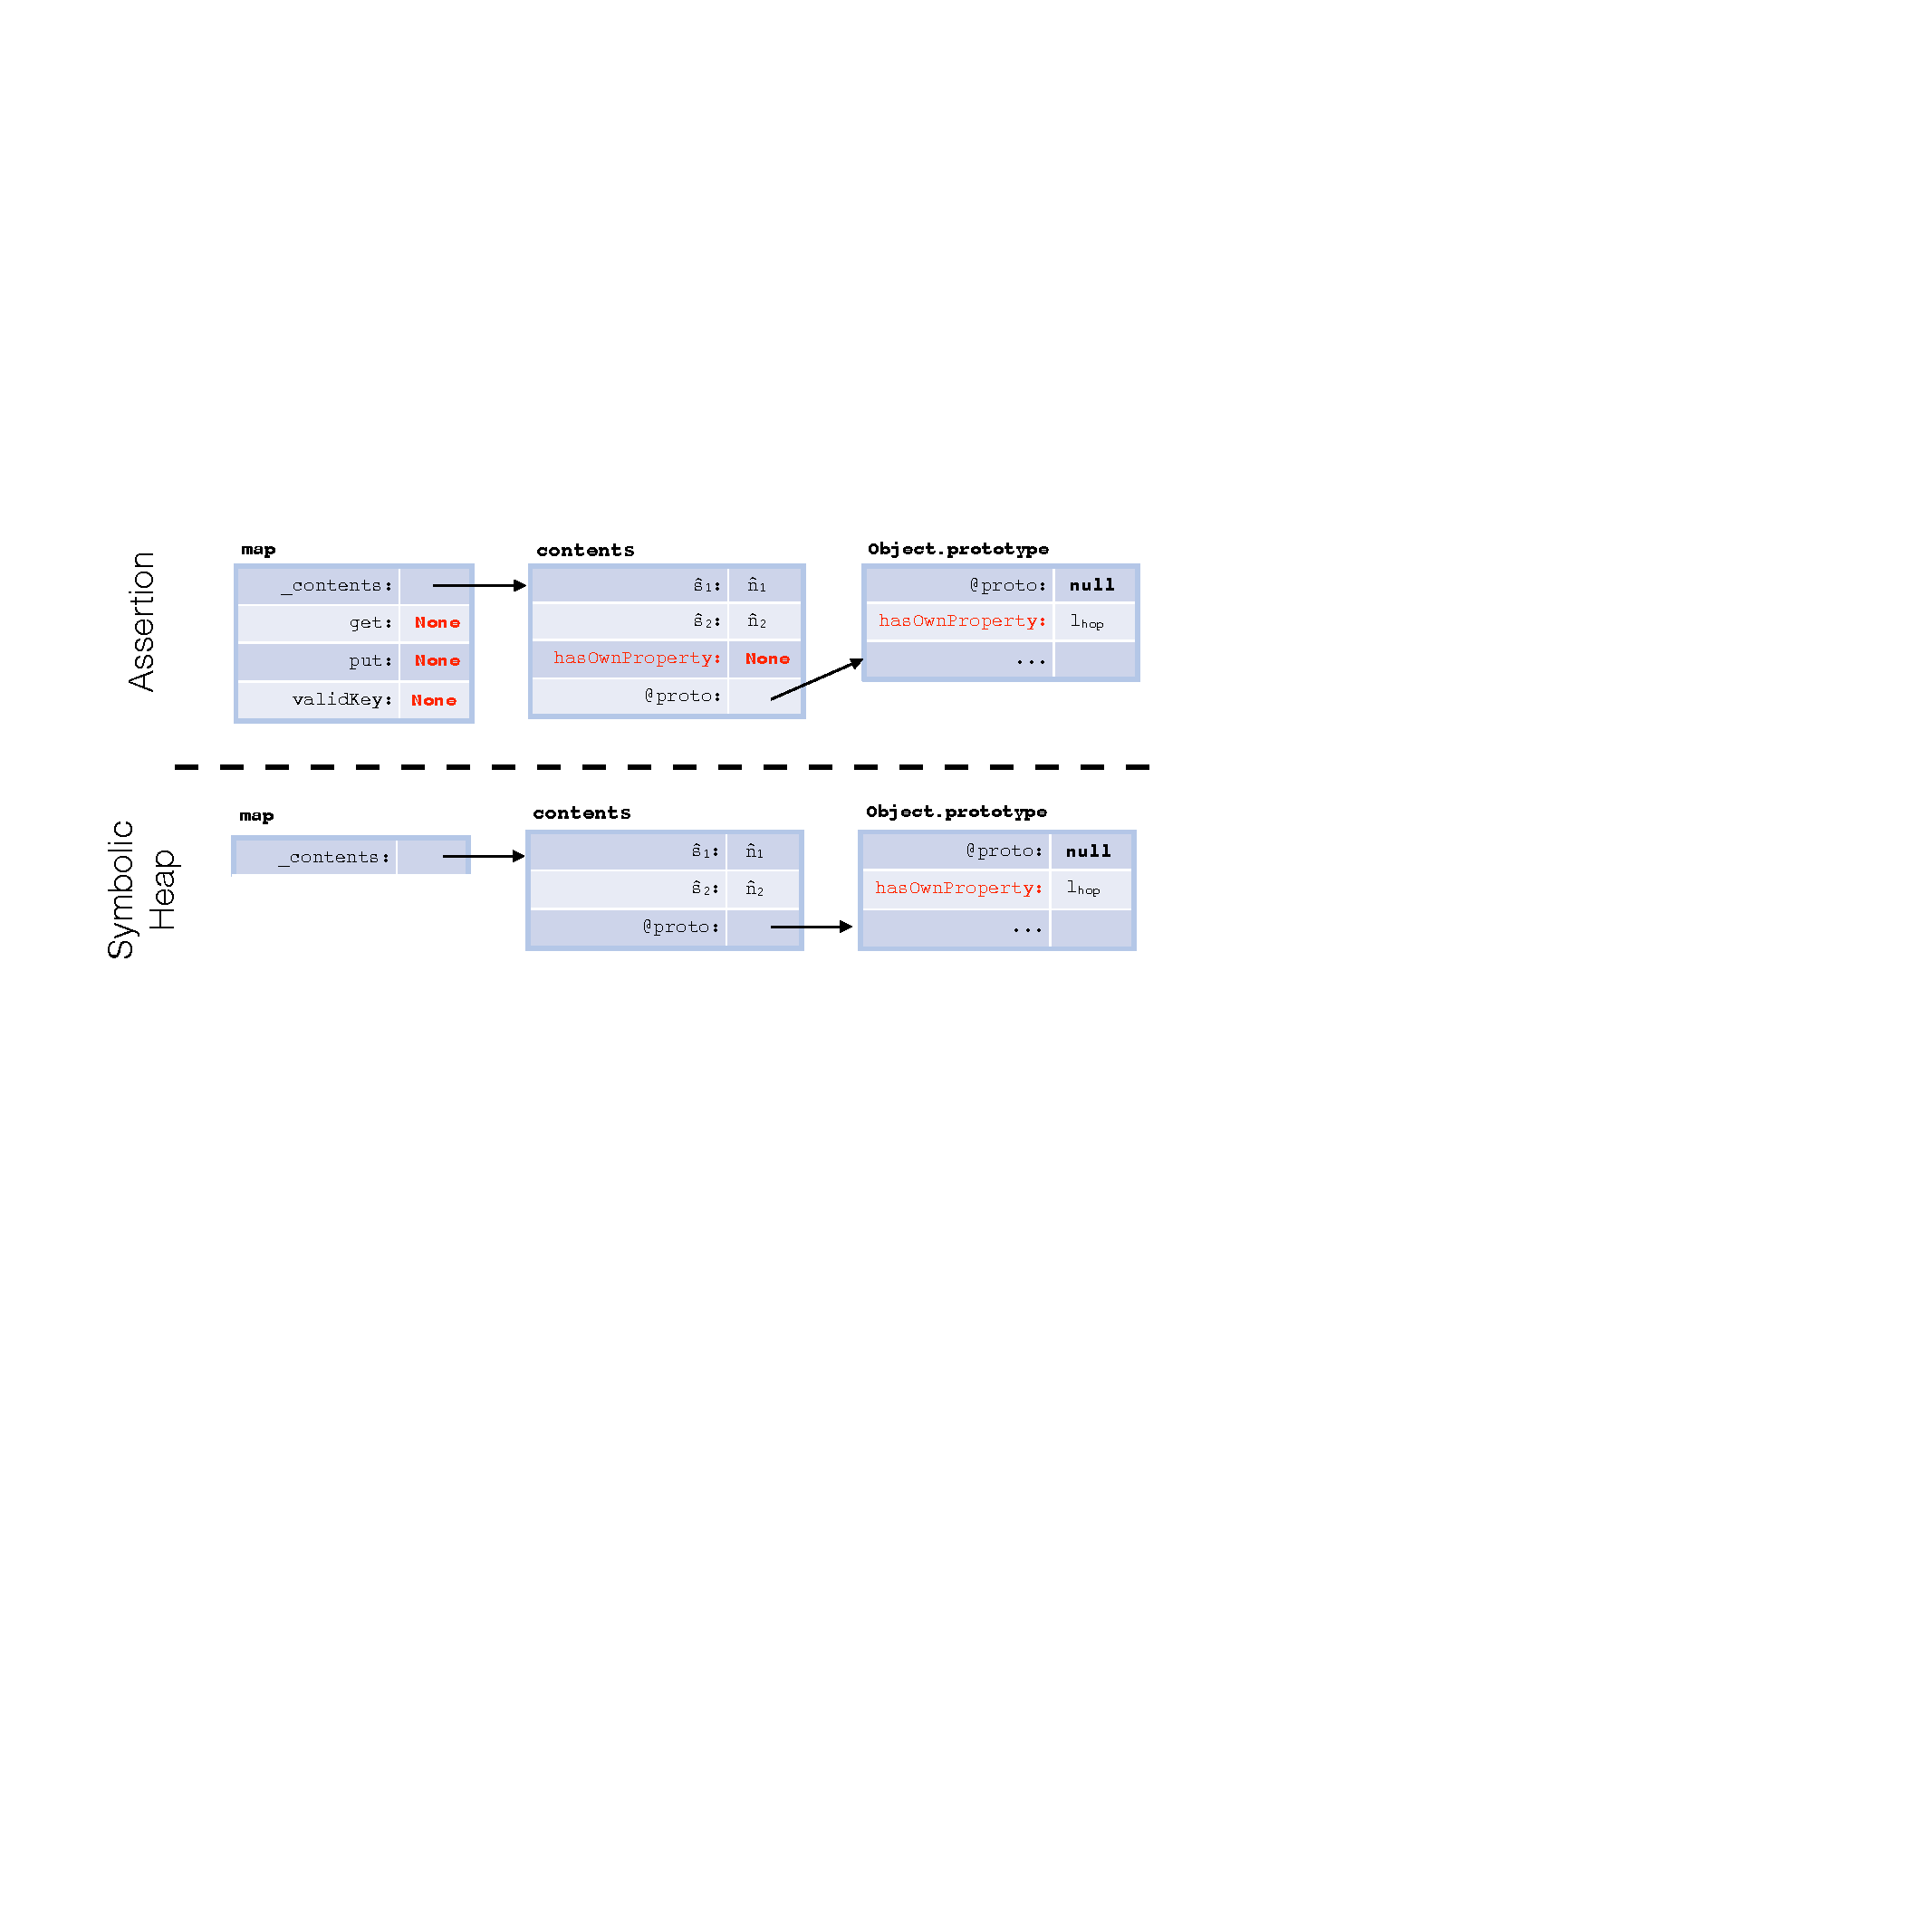
\includegraphics[width=0.9\textwidth]{figures/symbolicvsass.pdf}
{\small $$
\text{\emph{None-Constraints: }} (\hat{s}_1 \neq \texttt{"hasOwnProperty"} \, \wedge \, \hat{s}_2 \neq \texttt{"hasOwnProperty"})
$$}
\vspace{-25pt}
\caption{Assertion vs. Symbolic Heap}
\end{figure}



%\begin{algorithm}
%\caption{Synthesising a symbolic test for: $\lconf{P} \, \fid(\jvec{x}) \,  \lconf{Q}$}\label{infer:specs:algo}
%\begin{algorithmic}[1]
%\State $(\existentials, \sfs, \pfs) := \normalise(P)$ 
%\State $\sheap_0, \pfs_0, \theta := \concretise{(\existentials, \sfs, \pfs)}{[ \ ]}$
%\State $\subst' := \subst\mid_{\domain(\subst) \backslash \existentials}$
%\State Return: 
%%\ForAll{$XXX$}
%%\If{$XXX$}
%  %\State $\{ P \} \, \pid() \, \{ Q \} = \ispecs(\pid, \_)$
%%\Else
%  %\State $P,Q :=$
%%\EndIf
%%\State $ := InferSpec, \ispecs', \pid, P) $
%%\ForAll{$(Q_f,,\flag) \in $}
%%\If{$Q_f \sep Q_M \vdash Q \sep \true$}
%  %\State $\ispecs' := \ispecs' \cup \{(\pid, \flag) \mapsto {P \sep _f \sep Q_M}{\pid(\jvec{\xivar})}{Q_f \sep Q_M}\}$
%%\EndIf
%%\EndFor
%%\EndFor
%\end{algorithmic}
%\end{algorithm}


\subsection{Generating Symbolic Tests from JavaScript} 
\label{specs:example}

\myparagraph{Example}
In Figure~\ref{fig:map:example}, we define a \emph{map object predicate}, \jsinline|Map|, 
using the auxiliary predicate \jsinline|KVPairs|, which captures the resource of the key-value pairs in the map, 
and the \jsinline|validKey(k)| predicate, which holds if and only if the 
JavaScript function \jsinline|ValidKey(k)| returns \jsinline|true|\footnote{We treat the $\mathtt{ValidKey}$ predicate as a black box.}.
%
Intuitively, the \jsinline|Map(m, mp, kvs, keys)| predicate captures the resource 
of a map object \jsinline|m| with prototype \jsinline|mp|, keys \jsinline|keys| (a set of strings),
and key-value pairs \jsinline|kvs| (a set of string pairs\footnote{We model pairs as lists with two elements and, for clarity, use the pair notation.}). 
Observe that the definition of \jsinline|Map| does not include the resource of a map prototype, as
it is shared between all map objects, and therefore needs to be factored out.  
%
We write \jsinline|-u-| for set union and omit the brackets around singleton 
sets when the meaning is clear. % from the context. 

\begin{figure}[t!]
{\scriptsize
 \begin{verbatim}
Map (m, mp, kvs, keys) := JSObject(m, mp) * 
  DataProp(m, "_contents", c) * JSObject(c, Object.prototype) * KVPairs(c, kvs, keys) *
  (m, "get") -> None * (m, "put") ->  None * (m, "validKey") ->  None * 
  (c, "hasOwnProperty") ->  None *  emptyFields(c, keys -u- "hasOwnProperty")
  \end{verbatim}
  \vspace*{-0.3cm}
 \begin{verbatim}
KVPairs (o, kvs, keys) := 
  (kvs = { }) * (keys = { }),
  (kvs = (key, value) -u- kvs') * (keys = key -u- keys') * 
    ValidKey(key) * DataProp(o, key, value) * KVPairs(o, kvs', keys')
\end{verbatim}}
\caption{Map predicate \label{fig:map:example}}
\end{figure}

%In the following, we assume a \jsinline|MapProto| predicate specifying the resource of 
%a valid map prototype. In particular, the map prototype needs to define the methods 
%\jsinline|put|, \jsinline|get|, and \jsinline|validKey|. 


We are now in the position to specify the functions of the map library. In particular, below we show how to use 
the map object predicate to specify \jsinline|get(k)|.  
%
We consider the case in which the key whose value we  want to fetch is stored in the 
map.  The specification is given below. 
%
\begin{displaymath} 
{\footnotesize
\begin{array}{c}
\left\{ {\begin{array}{c}
 \text{\texttt{Map(this, mp, kvs -u- (k, v), ks) * ObjProtoF()}} \\ 
\end{array}} \right\} \\
%
\text{\bfseries \texttt{get(k)}} \\[0.2mm]
%
\left\{ {\begin{array}{c}
 \text{\texttt{Map(this, mp, kvs -u- (k, v), ks) * ObjProtoF() * (ret = v) }} \\
\end{array}} \right\}
\end{array}
} 
\end{displaymath}
%
The predicate \jsinline|ObjProtoF()| describes the resource captured by the \jsinline|Object.prototype| object. 
In particular, it is needed because \texttt{get} uses the \texttt{hasOwnProperty} function.



%%
%% OLD THINGS

%\begin{figure}[t!]
%\centering
%{\scriptsize
%\begin{mathpar} 
%\inferrule[\textsc{New Existential}]
%     { 
%         \svar \in \existentials 
%         \quad
%         \svar \not\in \domain(\subst)
%     }
%     {\unification{\sexpr, \pc}{\svar}{\subst}{\existentials} = \optionsome{\subst[\svar \mapsto \sexpr]}}
%\quad
%\inferrule[\textsc{Matched Existential}]
%     { 
%         \subst(\svar) = \sexpr' 
%         \quad 
%         \pc \vdash \sexpr = \sexpr' 
%     }
%     {\unification{\sexpr, \pc}{\svar}{\subst}{\existentials} = \optionsome{\subst}}
%\quad
%\inferrule[\textsc{Existential - None}]
%     { 
%         \subst(\svar) = \sexpr' 
%         \quad 
%         \pc \vdash \sexpr \neq \sexpr' 
%     }
%     {\unificationfail{\sexpr, \pc}{\svar}{\subst}{\existentials} = \optionnone}
%\\
%\inferrule[\textsc{Grounded Expression}]
%     { 
%         \fv(\subst(\sexpr')) \cap \existentials = \emptyset
%         \quad 
%          \pc \vdash  \sexpr = \subst(\sexpr') 
%     }
%     {\unification{\sexpr, \pc}{\sexpr'}{\subst}{\existentials} = \optionsome{\subst}}
%\qquad
%\inferrule[\textsc{Grounded Expression - Fail}]
%     { 
%         \fv(\subst(\sexpr')) \cap \existentials = \emptyset
%         \quad 
%          \pc  \vdash  \sexpr \neq \subst(\sexpr') 
%     }
%     {\unification{\sexpr, \pc}{\sexpr'}{\subst}{\existentials} = \optionnone}
%%
%\\
%\inferrule[\textsc{Cell Assertion}]
%	{  
%	   \big(\loc = \symbeval{\lexpr_l}{\sstore} \ \vee \loc = \subst(\symbeval{\lexpr_l}{\sstore}) \big)
%	   \quad 
%	     \symbeval{\lexpr_p}{\sstore} = \sexprp'
%	   \quad
%	   \symbeval{\lexpr_v}{\sstore} = \sexprv' 
%	   \quad
%	    \sheap = \sheap_f \dunion ((l, \sexprp) \mapsto \sexprv) 
%	   \\
%	   \unification{\sexprp, \pc}{\sexprp'}{\subst}{\existentials} = \optionsome{\subst'} 
%	   \quad
%	   \unification{\sexprv, \pc}{\sexprv'}{\subst'}{\existentials} = \optionsome{\subst''} 
%	}{ \unification{\sheap, \sstore, \pc}{(\lexpr_l,\lexpr_p)\pointsto \lexpr_v}{\subst}{\existentials} = \optionsome{(\subst'', \sheap_f)}} 
%\\
%\inferrule[\textsc{Cell Assertion - Fail}]
%	{  
%	   \big(\loc = \symbeval{\lexpr_l}{\sstore} \ \vee \loc = \subst(\symbeval{\lexpr_l}{\sstore}) \big)
%	   \quad
%	     \symbeval{\lexpr_p}{\sstore} = \sexprp'
%	   \quad
%	   \symbeval{\lexpr_v}{\sstore} = \sexprv' 
%	   \quad
%	     \sheap = \sheap' \dunion  \big((l, \sexprp_i) \mapsto \sexprv_i\big)\mid_{i = 0}^n   
%  	   \\
%	    (l, -) \not\in \domain(\sheap') 
%	    \quad 
%	   \forall_{0 \leq i \leq n} \, \unification{\sexprp, \pc}{\sexprp'}{\subst}{\existentials} = \optionnone 
%	   \ \vee \
%	   \unification{\sexprv, \pc}{\sexprv'}{\subst'}{\existentials} = \optionnone
%	}{ \unification{\sheap, \sstore, \pc}{(\lexpr_l,\lexpr_p)\pointsto \lexpr_v}{\subst}{\existentials} = \optionnone} 
%\\
%\inferrule[\textsc{EmptyFields Assertion}]
%	{  
%	   \big(\loc = \symbeval{\lexpr_l}{\sstore} \ \vee \loc = \subst(\symbeval{\lexpr_l}{\sstore}) \big)
%	   \quad 
%	     \symbeval{\lexpr_d}{\sstore} = \sexprv' 
%	   \\\\
%	     \sheap = \sheap' \, \uplus \, \big((l, \sexprp_i) \mapsto \sexprv_i\big)\mid_{i = 0}^n   
%              \quad
%             (l, -) \not\in \domain(\sheap')
%	    \quad 
%	    \pc \vdash \big( \{ \sexprp_i \mid_{i = 0}^n   \} \subseteq \sexprv' \big)
%	}{ \unification{\sheap, \sstore, \pc}{\emptyfields{\lexpr_l}{\lexpr_d}}{\subst}{\existentials} = \optionsome{(\subst, \sheap)}} 
%\\
%\inferrule[\textsc{EmptyFields Assertion - Failing}]
%	{  
%	   \big(\loc = \symbeval{\lexpr_l}{\sstore} \ \vee \loc = \subst(\symbeval{\lexpr_l}{\sstore}) \big)
%	   \quad 
%	     \symbeval{\lexpr_d}{\sstore} = \sexprv' 
%	   \\\\
%	     \sheap = \sheap' \, \uplus \, \big((l, \sexprp_i) \mapsto \sexprv_i\big)\mid_{i = 0}^n   
%              \quad
%             (l, -) \not\in \domain(\sheap')
%	    \quad 
%	    \pc \vdash \big( \{ \sexprp_i \mid_{i = 0}^n   \} \not\subseteq \sexprv' \big)
%	}{ \unification{\sheap, \sstore, \pc}{\emptyfields{\lexpr_l}{\lexpr_d}}{\subst}{\existentials} = \optionnone} 
%\end{mathpar}
%\hrule
%\caption{Unification of spatial assertions:
% {\scriptsize$\unification{\sheap, \sstore, \pc}{\cell}{\subst}{\existentials} = (\subst', \sheap_f)$}\label{fig:unification}}}
%\end{figure}


%{\small 
%\begin{align}
%\sepmodels{P} = \left\{ (\iheap, \store) \mid \exists \senv \, . \,  \iheap, \store, \senv \satisfies P  \right\} 
%\\ 
%\smodels{\isheap, \sstore}{\pc} = \left\{ (\iheap, \store) \mid \exists \senv \, . \,  \senv \vdash \pc \ \wedge \
%    \iheap = \symbeval{\isheap}{\senv} \ \wedge \ \store = \symbeval{\sstore}{\senv}  \right\} 
%\end{align}} 



%
%\begin{figure}
%{\scriptsize
%\centering
%\begin{mathpar} 
%\inferrule[\textsc{Spatial Assertion}]
%	{  
%	   \unification{\sheap, \sstore, \pc}{(\lexpr_l,\lexpr_p)\pointsto \lexpr_v}{\subst} = \uyes{\sheap_f}
%	}{\cellunification{\sheap, \cell \lstcons \cells}{\sheap_q, \cells}{\sstore, \pc, \subst}} 
%\\
%\inferrule[\textsc{Successful Unification}]
%	{  
%	   
%	   \cellunificationiter{\sheap, \cells}{\hemp, []}{\sstore, \pc, \subst}
%	   \qquad 
%	   \pc \vdash \subst(\pfs')
%%	   \cells =  \cell \lstcons \cells'
%%	   \and
%%            \unification{\sheap, \sstore, \pc}{\cell}{\subst} = \uyes{\sheap_f}
%%            \\\\
%%            \unificationfull{\sheap_f, \sstore, \pc}{\cells', \pfs'}{\subst}
%	}{\unificationfull{\sheap, \sstore, \pc}{\cells, \pfs'}{\subst}} 
%\and 
%\inferrule[\textsc{Spatial Assertion}]
%	{  
%	   \cells = \cell \lstcons \cells'
%	   \and
%            \unification{\sheap, \sstore, \pc}{\cell}{\subst} = \uyes{\sheap_f}
%            \\\\
%            \unificationfullfail{\sheap_f, \sstore, \pc}{\cells', \pfs'}{\subst}{\pc'}
%	}{\unificationfullfail{\sheap, \sstore, \pc}{\cells, \pfs'}{\subst}{\pc'}} 
%\\
%\inferrule[\textsc{Pure Assertions}]
%	{  
%	   \pc \vdash \subst(\pfs')
%	}{\unificationfull{\hemp, \sstore, \pc}{\emptyset, \pfs'}{\subst}} 
%%
%\and
%%
%\qquad
%\inferrule[\textsc{Pure Assertions -  Fail}]
%	{  
%	      \pc \not\vdash \subst(\pfs')
%	}{\unificationfullfail{\sheap, \sstore, \pc}{\emptyset, \pfs'}{\subst}{\subst(\pfs')}} 
%\\
%%
%\inferrule[\textsc{Cell Assertion - Fail}]
%	{  
%	   \sfs = \cells \lstcons \cells
%	   \and
%            \unification{\sheap, \sstore, \pc}{\cell}{\subst} = \uno{\pc'}
%	}{\unificationfullfail{\sheap, \sstore, \pc}{\sfs, \pfs'}{\subst}{\pc'}} 
%%
%\and
%\inferrule[\textsc{Extra Resource -  Fail}]
%	{  
%	    \sheap \neq \hemp
%	}{\unificationfullfail{\sheap, \sstore, \pc}{\emptyset, \pfs'}{\subst}{\jtrue}} 
%%
%\end{mathpar}}
%\hrule

